%%%%%%%%%%%%%%%%%%%%%%%%%%%%%%%%%%%%%%%%%
% University Assignment Title Page 
% LaTeX Template
% Version 1.0 (27/12/12)
%
% This template has been downloaded from:
% http://www.LaTeXTemplates.com
%
% Original author:
% WikiBooks (http://en.wikibooks.org/wiki/LaTeX/Title_Creation)
%
% License:
% CC BY-NC-SA 3.0 (http://creativecommons.org/licenses/by-nc-sa/3.0/)
% 
% Instructions for using this template:
% This title page is capable of being compiled as is. This is not useful for 
% including it in another document. To do this, you have two options: 
%
% 1) Copy/paste everything between \begin{document} and \end{document} 
% starting at \begin{titlepage} and paste this into another LaTeX file where you 
% want your title page.
% OR
% 2) Remove everything outside the \begin{titlepage} and \end{titlepage} and 
% move this file to the same directory as the LaTeX file you wish to add it to. 
% Then add \input{./title_page_1.tex} to your LaTeX file where you want your
% title page.
%
%%%%%%%%%%%%%%%%%%%%%%%%%%%%%%%%%%%%%%%%%
%\title{Title page with logo}
%----------------------------------------------------------------------------------------
%	PACKAGES AND OTHER DOCUMENT CONFIGURATIONS
%----------------------------------------------------------------------------------------

\documentclass[12pt]{article}

\usepackage[francais]{babel}
\usepackage[utf8x]{inputenc}
\usepackage[T1]{fontenc}
\usepackage{color}

\usepackage{amsmath}
\usepackage{graphicx}
\usepackage{enumerate}

% Define new command
\newcommand{\HRule}{\rule{\linewidth}{0.5mm}}

\newcommand{\crt}{\emph{Nexys 4 DDR\ }}
%\def\thesubsection{\alph{section}}

\begin{document}

\begin{titlepage}

\center % Center everything on the page
 
%----------------------------------------------------------------------------------------
%	HEADING SECTIONS
%----------------------------------------------------------------------------------------

\textsc{\LARGE Universit\'e Pierre et Marie Curie}\\[1.5cm] % Name of your university/college
\textsc{\Large PSESI}\\[0.5cm] % Major heading such as course name

%----------------------------------------------------------------------------------------
%	TITLE SECTION
%----------------------------------------------------------------------------------------

\HRule \\[0.4cm]
{ \huge \bfseries Rapport de pr\'e-soutenance}\\[0.4cm] % Title of your document
{ \huge \bfseries D\'eveloppement sur FPGA \\d'un système d'aiguillage
  \\pour centale DCC sur train miniature}\\[0.4cm] % Title of your document
\HRule \\[1.5cm]
 
%----------------------------------------------------------------------------------------
%	AUTHOR SECTION
%----------------------------------------------------------------------------------------

\begin{minipage}{0.4\textwidth}
\begin{flushleft} \large
\emph{\'Etudiant:}\\
Maxime \textsc{AYRAULT} 3203694 % Your name
\end{flushleft}
\end{minipage}
~
\begin{minipage}{0.4\textwidth}
\begin{flushright} \large
\emph{Encadrant:} \\
Julien \textsc{DENOULET} % Supervisor's Name
\end{flushright}
\end{minipage}\\[2cm]

%----------------------------------------------------------------------------------------
%	DATE SECTION
%----------------------------------------------------------------------------------------

{\large \today}\\[2cm] % Date, change the \today to a set date if you want to be precise

%----------------------------------------------------------------------------------------
%	LOGO SECTION
%----------------------------------------------------------------------------------------

%%\begin{figure}
%%  \subfigure[]{
\includegraphics[scale=0.2\textwidth]{logo.png}} 
%%\end{figure} 

\includegraphics[width=0.2\textwidth]{logo.png}

%----------------------------------------------------------------------------------------

\vfill % Fill the rest of the page with whitespace

\end{titlepage}



\begin{abstract}
Your abstract here.
\end{abstract}

\section{Introduction}
\label{sec:introduction}

\subsection{\underline{ Contexte et encadrement}}

Depuis plusieurs ann\'ees, le laboratoire lip6 d\'eveloppe un projet de
gestion de maquettes de trains. Ce projet se base sur une
\emph{centrale DCC}. Cette centrale permet de recevoir la position des
trains et des aiguilles et d'envoyer des commandes en utilisant le
\emph{protocole DCC}.

Ce projet est r\'ealis\'e seul et est encadr\'e par le Responsable de la
valuer FPGA. Ce projet se d\'eroule sur une dur\'ee de 6 semaines.
Il est r\'ealis\'e dans le cardre d'un projet SESI.

\subsection{\underline{Objectifs}}

L'objectif de mon projet consiste, dans un premier temps, à porter la
\emph{centrale DCC} implement\'ee par d'autres \'etudiants sur une nouvelle
carte mat\'eriel \emph{FPGA}. La version courante de la centrale tourne sur
une carte \emph{Spartan 6}, elle est remplac\'ee par notre \crt qui est
une carte plus r\'ecente et possède une interface plus complète
\emph{(switchs, boutons, afficheurs 7 segments...)}
Dans un second temps, mon projet consiste à ajouter la commande de
des aiguillages.

Je propose par commencer par une gestion manuelle des aiguillages avec
les diff\'erents switchs de la carte sans v\'erification de s\'ecurit\'e. Puis
une fois cela fait, je vais impl\'ementer par une gestion des
enclenchements ferroviaire grâce aux differents capteurs pr\'esents sur
les rails. Ceci permet de garantir qu'un train ne devra pas pouvoir
changer de voie que si aucun autre train ne se trouve sur le chemin
qu'il veut parcourir. 

Les domaines de comp\'etences requis sont multiples; la connaissance
du langage VDHL et de la plateforme \emph{FPGA} pour l'impl\'ementation
de la centrale DCC et la connaissance de la gestion des enclenchements
ferroviaires.


\newpage
\section{Aspects techniques}
\label{sec:asp_tech}

\subsection{\underline{ Le protocole DCC}}
\label{sec:dcc}


\begin{figure}[ht]
\centering
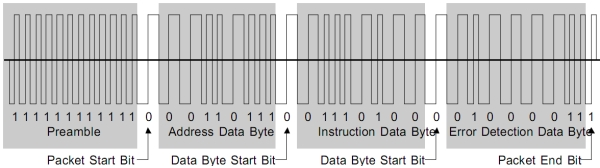
\includegraphics[scale=0.75]{trame.png}
\caption{Exemple d'une trame DCC}
\label{fig1}
\end{figure}


Ce protocole est un protocole standardis\'e qui permet communiquer
entre ma cartec\emph{FPGA} et les diff\'erents trains et
composants. Il utilise une suite de commandes envoy\'ees sur les rails
jusqu'aux diff\'erents trains et composants qui agisent en fonction de
ce qu'ils recoivent.
Notre locomotive peut recevoir enormement de commandes différentes,
klason, annonces d'entr\`ee de gare, phares...(voir datasheet
locomotive) mais elles ne seront pas toutes implement\'ee ici, mais
pourront \^etre rajout\'e plus tard par la suite. 

\subsection{\underline{ La logique d'enclenchement}}
\label{sec:log_ixl}


\begin{figure}[ht]
\centering
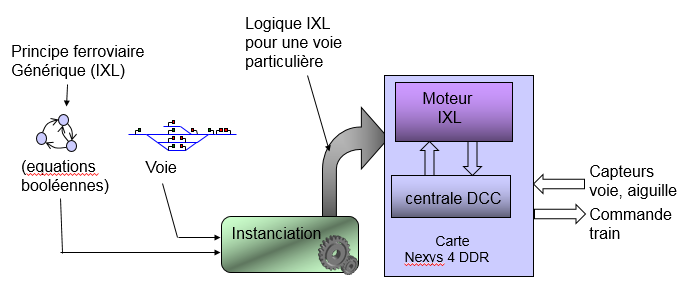
\includegraphics[scale=0.30]{moteur.png}
\caption{sch\'ema du moteur de gestion du circuit}
\label{fig2}
\end{figure}

\newpage

Un système ferroviaire est compos\'e de plusieurs systèmes :
\begin{itemize}
  \item Les \'equipements de voie (rails, aiguillages...) et le mat\'eriel
    roulant. C'est la partie visible des passagers
  \item Le Poste de Commande ferroviaire qui permet à un op\'erateur de
    visualiser, en temps r\'eel, l'\'etat du système (position des trains,
    position des aiguilles...
  \item La logique d'enclenchement qui assure la s\'ecurit\'e du système
    ferroviaire. Il est plac\'e entre le Poste de Commande ferroviaire
    et les \'equipements de voie. Il interdit les commandes lorsque les
    conditions incompatibles avec la s\'ecurit\'e. 
\end{itemize}




La figure suivante pr\'esente les relations entre les diff\'erents
systèmes.\emph{(voir fig3)}

\begin{figure}[ht]
\centering
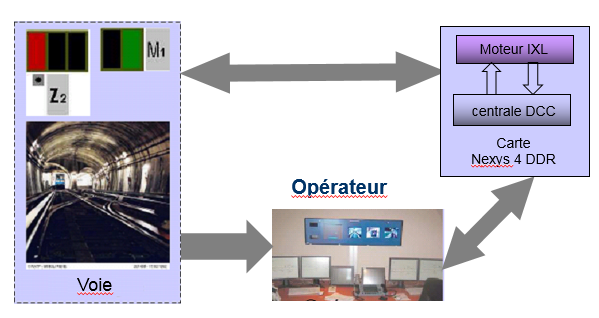
\includegraphics[scale=0.30]{sys_ferro.png}
\caption{relation entre les differents systemes}
\label{fig3}
\end{figure}


EXPLICATIONS....

\newpage

\subsection{\underline{ Architecture g\'en\'erale}}
\label{sec:archi}

  Voici un sch\'ema repr\'esentant l'installation que je vais
utiliser tout au long de mon projet.


\begin{figure}[ht]
\centering
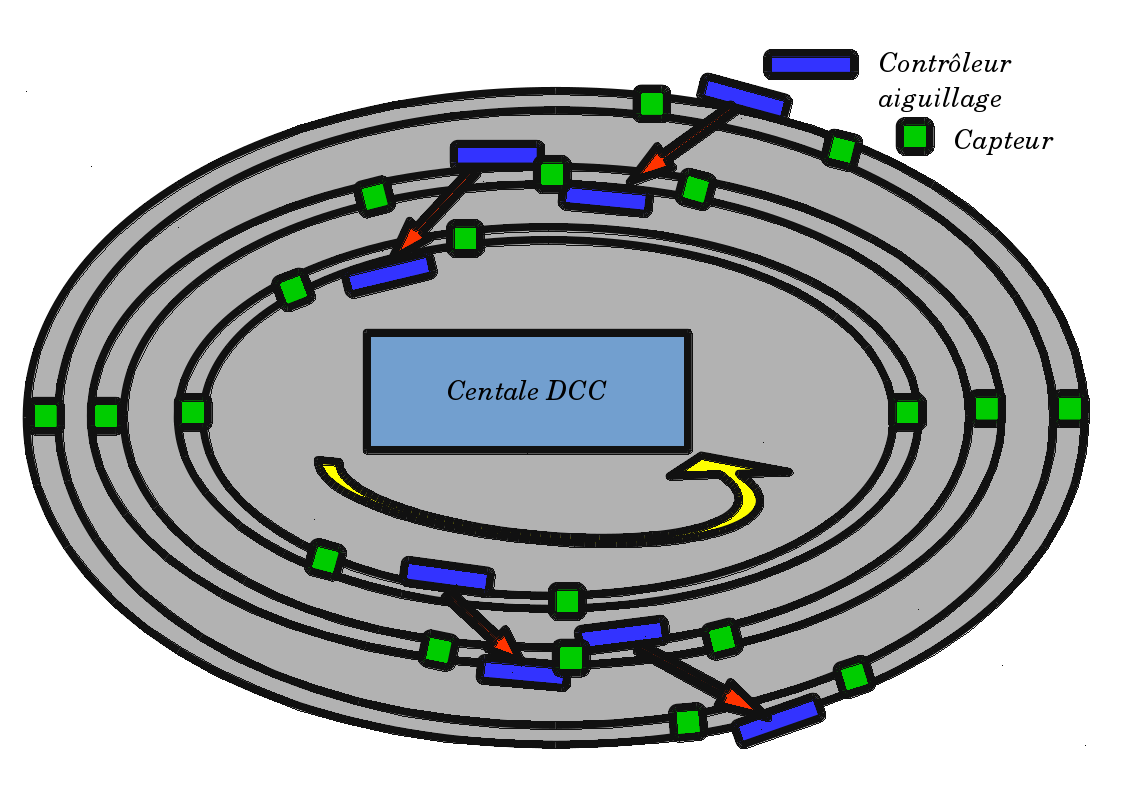
\includegraphics[scale=0.30]{schema.png}
\caption{sch\'ema de l'installation}
\label{fig4}
\end{figure}

  Notre installation\emph{(voir fig 4)} est donc compos\'e de 3 rails, de 6 aiguillages
control\'es par 8 contr\^oleurs gérés par trame DCC, et de 20 capteurs.
Le dispositif peut acceuillir jusqu'\`a 6 trains en m\^eme temps.

\begin{figure}[ht]
\centering
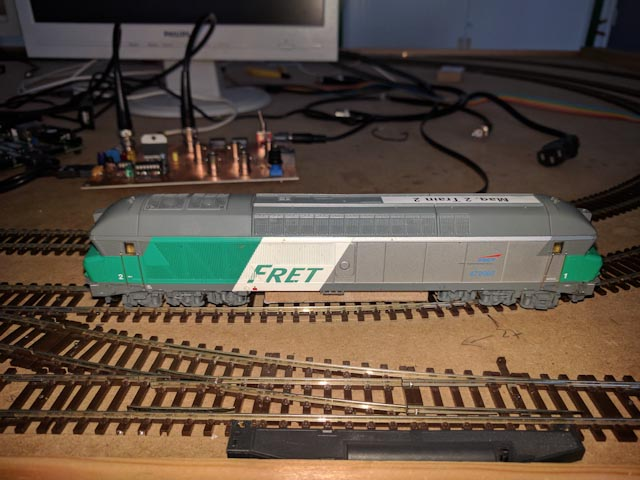
\includegraphics[scale=0.05]{loco.jpg}
\caption{photo de la locomotive}
\label{fig5}
\end{figure}

  Chaque locomotive poss\`ede une adresse sous forme de \emph{code
  barre} sous elle.\emph{(voir fig 6)}.
Le code \barre est decompos\'e de la façon suivante :
\begin{itemize}
    \item \textbf{un pr\`eambule} compos\'e de 2 bandes noires
      s\'epa\'ees par 1 bande blanche.
    \item \textbf{de l'adresse} le nombre de bandes noires correspond
      à l'adresse du train. 
    \item \textbf{un  \'epilogue} compo\'e de 3 bandes noires
      s\'epar\'ees par 2 bandes blanche.
\end{itemize}

\begin{figure}[ht]
\centering
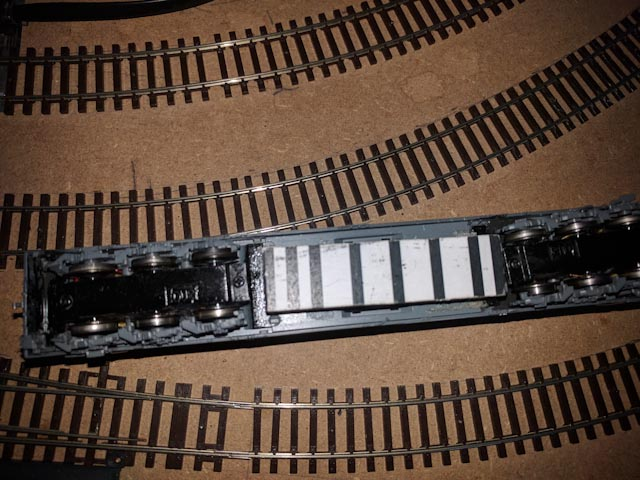
\includegraphics[scale=0.05]{add.jpg}
\caption{photo de l'adresse sous la locomotive}
\label{fig6}
\end{figure}

\newpage


\subsection{\underline{ Outils}}
\label{sec:outils}

Lors de ce projet, je vais devoir utiliser diff\'erents outils :
\begin{itemize}
  \item La carte \crt comme plateforme de d\'eveloppement
  \item La locomotive \emph{Jouef ``Fret SNCF``}\cite{Jouef}  et les capteurs de
    position et des aiguillages
  \item Le protocole DCC \cite{DCC}
  \item Le logiciel Vivado comme \emph{IDE}
\end{itemize}

ainsi que plusieurs langages:
\begin{itemize}
  \item \emph{VHDL}\cite{VHDL} comme language de description pour mes diff\'erentes
    \emph{IP}
  \item \emph{GIT}\cite{GIT} pour la gestion de configuration des logiciels
  \item \emph{\LaTeX}\cite{LATEX} pour la r\'edaction de la documentation
  \item Le langage \emph{Ocaml}\cite{OCAML} pour la g\'en\'eration de la logique d'enclenchement
\end{itemize}


\subsection{\underline{ Validation}}
\label{sec:valid}

Afin de tester et valider les differentes \'etapes de mon projet je vais
devoir faire des \emph{bancs de tests}, des simulations ainsi que des
exp\'erimentations qui pourront me permettre de valider mes essais.

Il y a d'ailleurs plusieurs sc\'enarios que je vais devoir r\'ealiser qui
me permettrons de tester de façon r\'eelle le fonctionnement de mes travaux.

En voici quelques un:

\begin{enumerate}[A]
  \item Sans Capteurs
  \begin{itemize}
    \item 1 train doit passer de la voie ``A`` à la voie ``B``
    \item 2 trains sur la voie ``A``, un seul doit passer sur la voie
       ``B``
  \end{itemize}

  \item Avec Capteurs
  \begin{itemize}
    \item 1 train doit passer de la voie ``A`` à la voie ``B``
    \item 2 trains sur la voie ``A``, un seul doit passer sur la voie ``B``
    \item 2 trains sur la voie 1 avec 1 seul qui doit passer de voie 1 à voie 2
    \item 1 train A sur voie 2 qui s'arrête dans la zone aiguillage.
    \item 1 train B sur voie 1 qui veut passer en voie 2 --> Pas
       possible. Red\'emarrage train A, v\'erification du changement de
       voie du train B.
  \end{itemize}
\end{enumerate}

\section{Organisation du projet}
\label{sec:org_proj}

\subsection{\underline{ Activit\'es du projet}}
\label{sec:activ}

Comme dit plus haut \emph{(voir 2.5)} le projet va \^etre decoup\'e en
plusieurs \'etapes diff\'erentes.

\begin{enumerate}[1]
  \item Avant aiguillage
  \begin{itemize}
    \item Dans un premier temps il faut cr\'eer une nouvelle interface
      homme machine
    \item Puis porter le code de l'ancienne centrale DCC et de la
      gestion des capteurs dans mon projet
    \item Et rajouter la gestion de l'aiguillage
  \end{itemize}

  \item Avec aiguillages
  \begin{itemize}
    \item Une fois l'aiguillage cr\'ee, il va falloir ajo\^uter la
      gestion des routes avec les différents switchs
    \item Puis pouvoir premettre de changer un aiguillage de place
      pour faire changer de voie un train uniquement avec les switchs
      sans aucun controle de s\'ecurit\'e.
    \item Et enfin de r\'ealiser les diff\'erents sc\'enarios decrit
      plus haut \emph{(voir 2.5)}
  \end{itemize}

  \item Avec aiguillages et capteurs
    \begin{itemize}
      \item Maintenant que j'ai la gestion de l'aiguillage et
        l'aquisition des différents capteurs je vais pouvoir rajouter
        de la s\'ecurit\'ee dans le systeme pour le rendre plus s\^ur.
      \item Je vais devoir rajouter un moteur XIL qui v\'erifira
        l'\'etat des voies avant de valider l'envoie d'une commande \`a
        un train.
      \item Et \`a la fin de mon projet je vais devoir r\'ealiser les
        diff\'erents sc\'enarios decrit plus haut \emph{(voir 2.5)}
        qui permeterons de valider les demandes de mon projet.      
    \end{itemize}
\end{enumerate}

\newpage

\subsection{\underline{ Planning pr\'evisionnel}}
\label{sec:planning}

  Voici les différentes taches ainsi que le planning que je compte
respecter pour reussir à mener à bien mon projet.


\begin{figure}[ht]
\centering
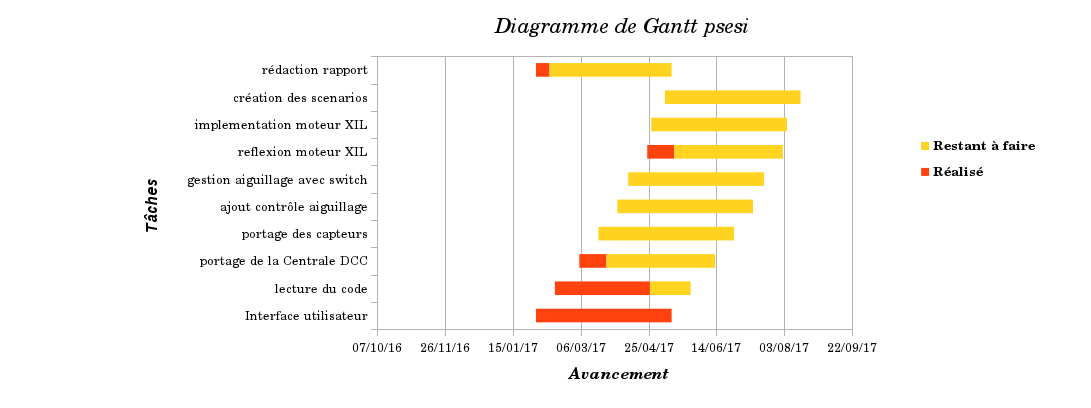
\includegraphics[scale=0.5]{gantt.png}
\caption{Diagramme de Gantt}
\label{fig6}
\end{figure}

\subsection{\underline{ Avancement}}
\label{sec:avanc}

J'ai d\'ej\`a commenc\'e \`a travailler sur le projet en essayant de
creer une ihm pour la s\'election des differentes valeurs que l'on
veut envoyer, 
  \begin{itemize}
    \item le choix de \textbf{l'adresse} du \emph{train} qui va recevoir la commande.
    \item le choix de \textbf{la vitesse} que \emph{le train} s\'electionn\'e
      va recevoir.
    \item le choix de \textbf{du numéro} de \emph{l'aiguillage} qui bougera.
    \item le choix de \textbf{la feature} qui pourra \^etre rajout\'ee
      au projet.
  \end{itemize}

\begin{figure}[ht]
    \begin{minipage}[c]{.46\linewidth}
        \centering
        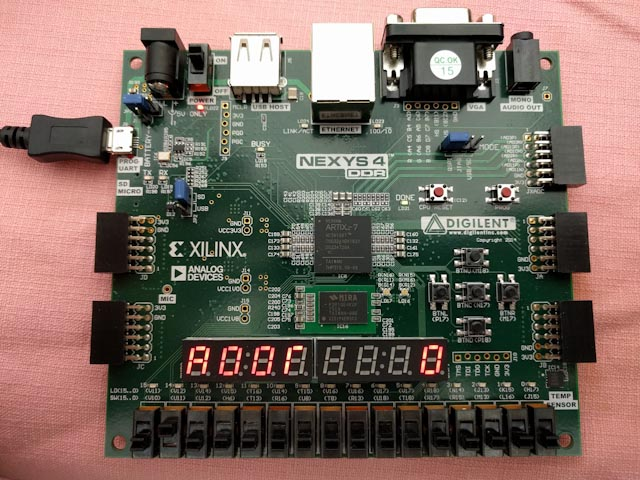
\includegraphics[scale=0.25]{exe_add.jpg}
        \caption{exemple d'utilisation de la carte}
        \label{fig7}
    \end{minipage}
    \hfill%
    \begin{minipage}[c]{.46\linewidth}
        \centering
        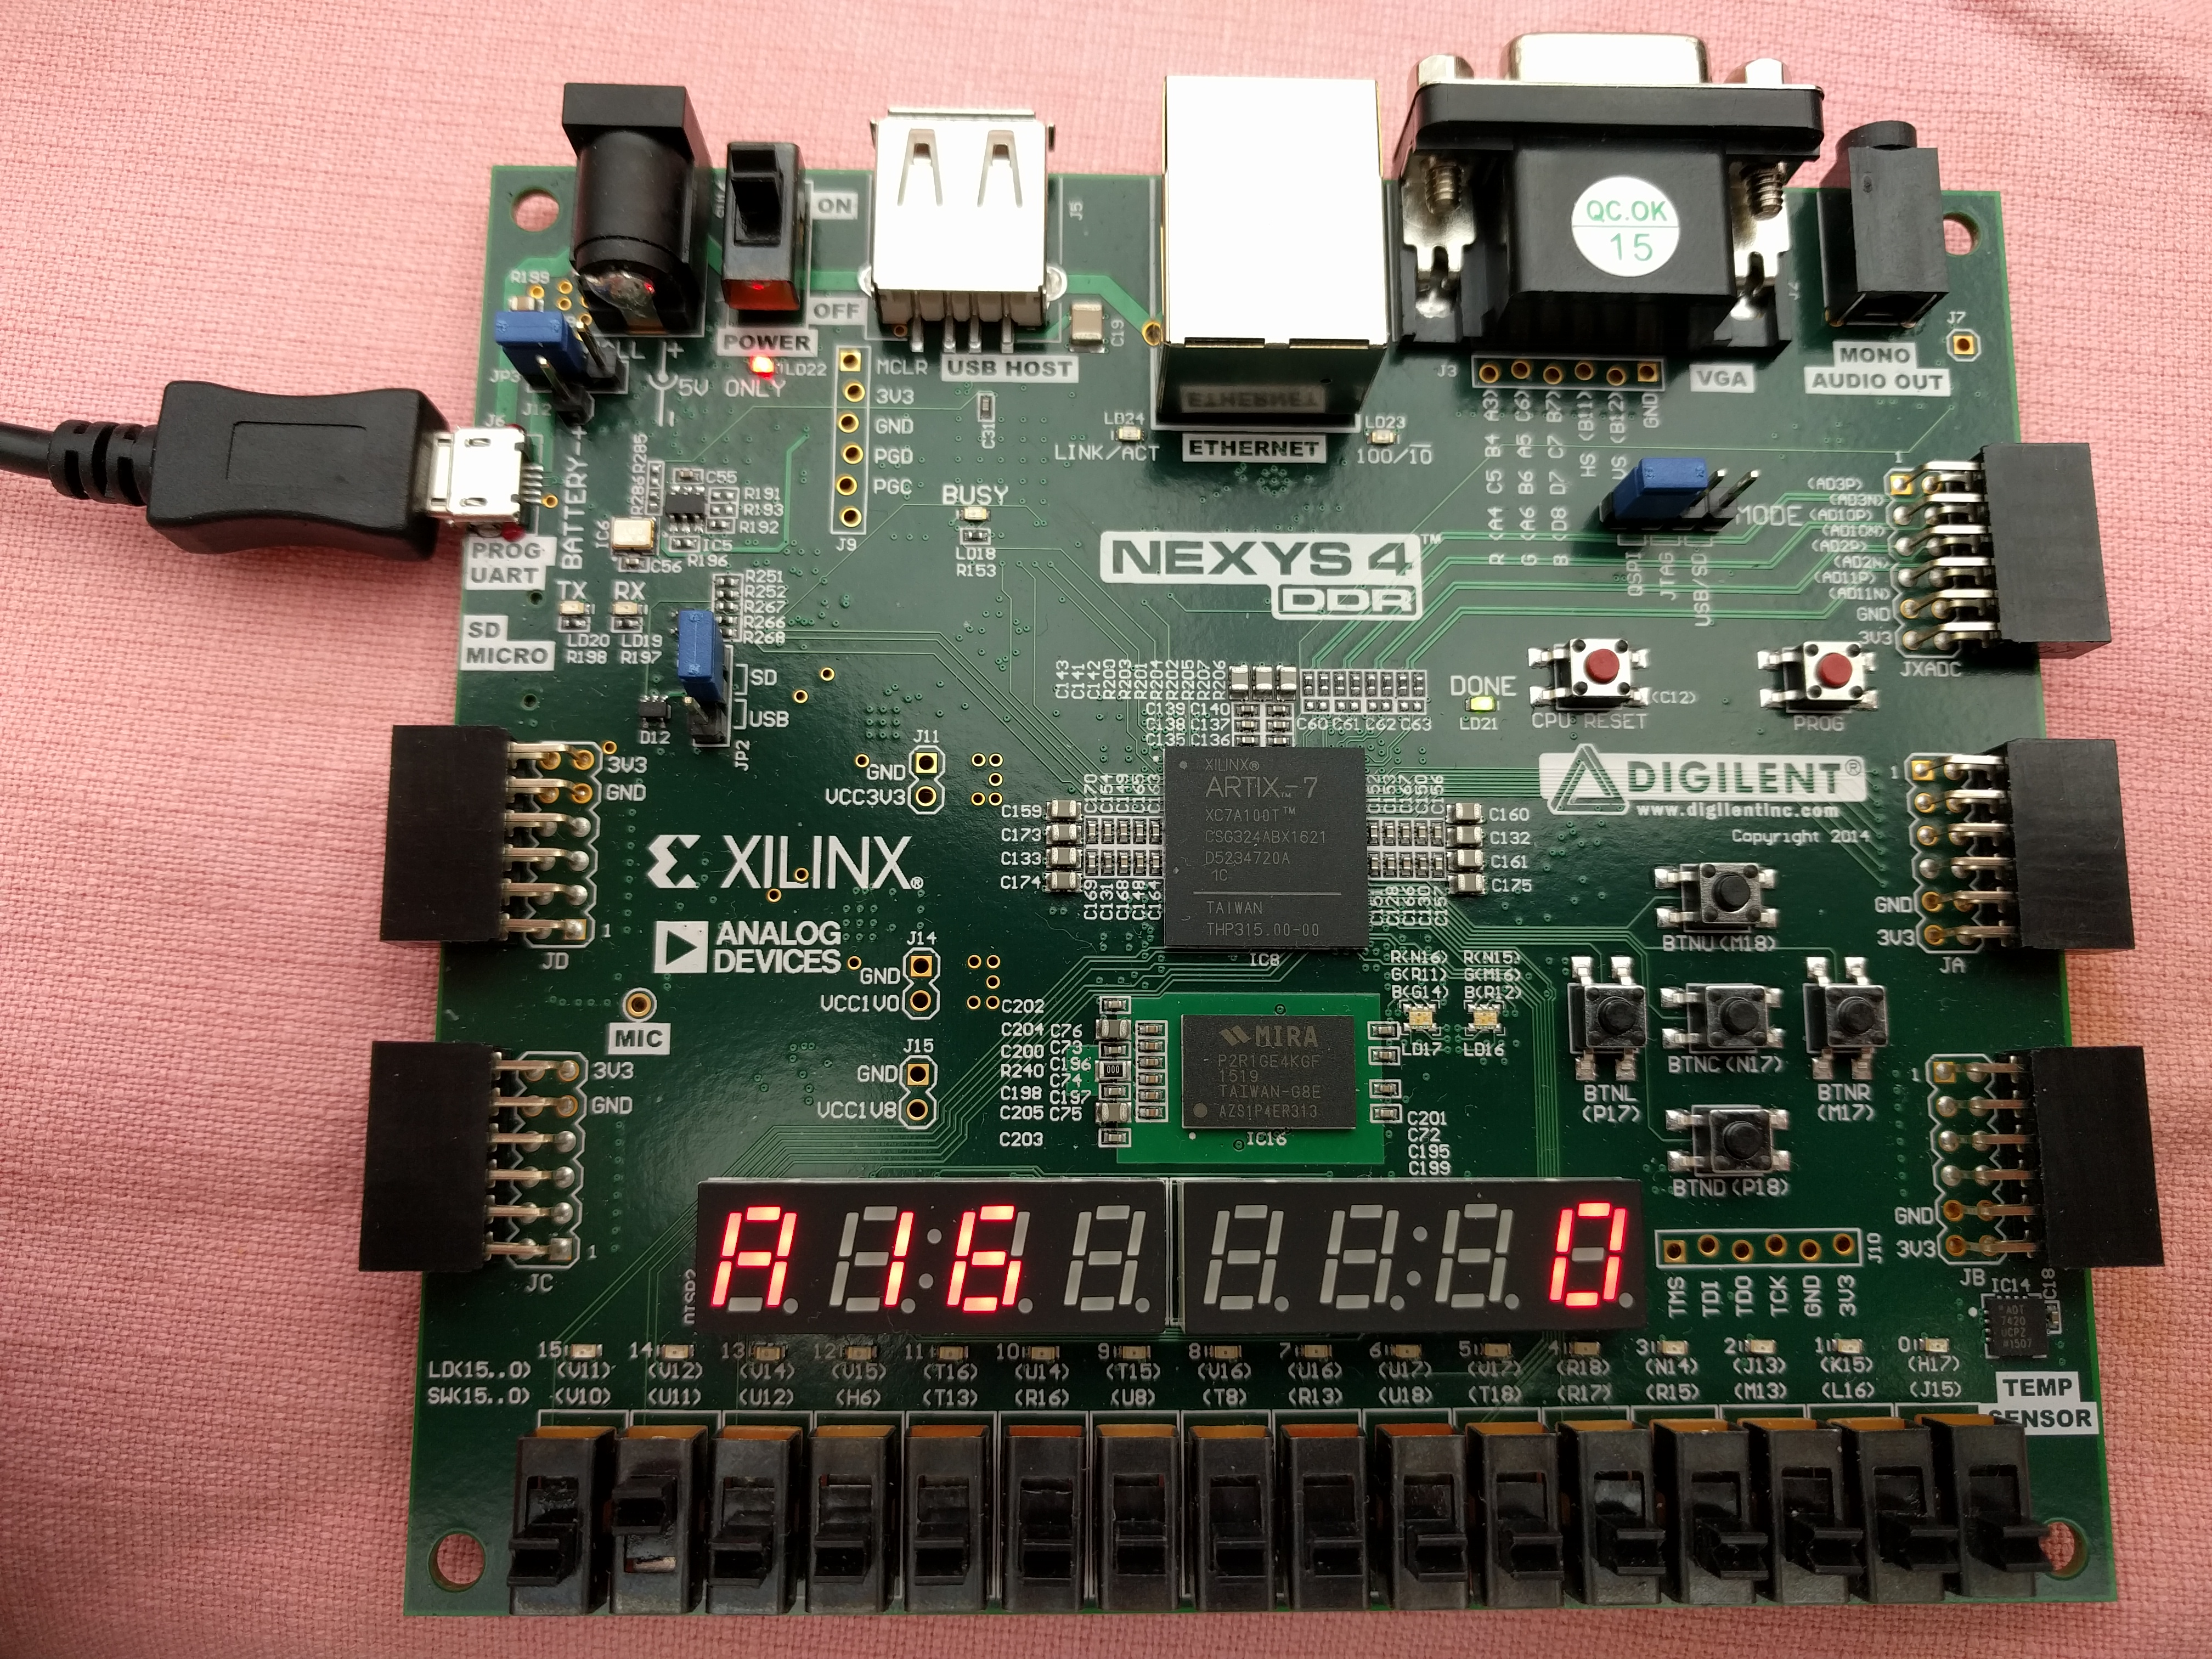
\includegraphics[scale=0.25]{exe_aigui.jpg}
        \caption{exemple d'utilisation de la carte}
        \label{fig8}
    \end{minipage}
\end{figure}

La \emph{figure 7} et la \emph{figure 8} sont un exemple du rendu de
mon ihm.

Je suis actuellement entrain de finir de porter le code de l'ancienne
centrale DCC et de l'aquisition des capteurs sur la nouvelle carte.

\newpage

\bibliographystyle{plain}
\bibliography{biblio}

\end{document}
